%%%%%%%%%%%%%%%%%%%%%%%%%%%%%%%%%%%%%%%%%%%%%%%%%%%%%%%%%%%%%%%%%%%%%%%%%%%%%%%%
%2345678901234567890123456789012345678901234567890123456789012345678901234567890
%        1         2         3         4         5         6         7         8

\documentclass[letterpaper, 10 pt, conference]{ieeeconf}  % Comment this line out
                                                          % if you need a4paper
%\documentclass[a4paper, 10pt, conference]{ieeeconf}      % Use this line for a4
                                                          % paper

\IEEEoverridecommandlockouts                              % This command is only
                                                          % needed if you want to
                                                          % use the \thanks command
\overrideIEEEmargins
% See the \addtolength command later in the file to balance the column lengths
% on the last page of the document



% The following packages can be found on http:\\www.ctan.org
%\usepackage{graphics} % for pdf, bitmapped graphics files
%\usepackage{epsfig} % for postscript graphics files
%\usepackage{mathptmx} % assumes new font selection scheme installed
%\usepackage{times} % assumes new font selection scheme installed
%\usepackage{amsmath} % assumes amsmath package installed
%\usepackage{amssymb}  % assumes amsmath package installed
\usepackage[cmex10]{amsmath}
%\usepackage[belowskip=-4pt, aboveskip=-0pt]{caption}
\usepackage{graphics} % for pdf, bitmapped graphics files
\usepackage{epsfig} % for postscript graphics files
\usepackage{epstopdf}
\usepackage{subfig}
\usepackage{mathptmx} % assumes new font selection scheme installed
\usepackage{times} % assumes new font selection scheme installed
\usepackage{amsmath} % assumes amsmath package installed
\usepackage{amssymb}  % assumes amsmath package installed
\usepackage{algorithmic}
\usepackage{array}
\usepackage{bm}
\usepackage{cite}
\title{\LARGE \bf
{Vision guided learning based bimanual robot sewing}
}

%\author{ \parbox{3 in}{\centering Huibert Kwakernaak*
%         \thanks{*Use the $\backslash$thanks command to put information here}\\
%         Faculty of Electrical Engineering, Mathematics and Computer Science\\
%         University of Twente\\
%         7500 AE Enschede, The Netherlands\\
%         {\tt\small h.kwakernaak@autsubmit.com}}
%         \hspace*{ 0.5 in}
%         \parbox{3 in}{ \centering Pradeep Misra**
%         \thanks{**The footnote marks may be inserted manually}\\
%        Department of Electrical Engineering \\
%         Wright State University\\
%         Dayton, OH 45435, USA\\
%         {\tt\small pmisra@cs.wright.edu}}
%}

\author{
\thanks{}
}

%\usepackage{caption}
%\setlength{\intextsep}{5pt plus 0pt minus 0pt}
\begin{document}

\maketitle
\thispagestyle{empty}
\pagestyle{empty}

%%%%%%%%%%%%%%%%%%%%%%%%%%%%%%%%%%%%%%%%%%%%%%%%%%%%%%%%%%%%%%%%%%%%%%%%%%%%%%%%
\begin{abstract}

\end{abstract}

%%%%%%%%%%%%%%%%%%%%%%%%%%%%%%%%%%%%%%%%%%%%%%%%%%%%%%%%%%%%%%%%%%%%%%%%%%%%%%%%


\section{Introduction}

%\begin{enumerate}
%\item{1} Bimanual manipulation-suturing is important and challenging
%\item{2} Our task is stent graft manufacturing
%%\item{3} Unsolved problems:Path planning,Adaptive to new context
%%\item{4} Our solutions:Vision + learn from demonstration,
%%Path planning - learning from demonstration, needle tracking, tool tracking,
%%Adaptive to new context - object centric approach + vision guided.
%\end{enumerate}
%~\cite{bidan2013grasp}

Stent grafts are tubular shape implants for supporting diseased vessels caused by abdominal aortic aneurysm (AAA). Generally, stent grafts comprise two components: a quasi blood-tight textile tube called graft and a reinforcing metallic ring called stent. Clinically, each stent graft needs to be customised to the patient anatomy, with fenestrations (openings) on the graft body to maintain the patency of important branches to vital organs. Generally, hand sewing techniques are used to attach the reinforcing rings to the fabric and finishing the edge of a fenestration. It is very similar with the suturing technique used in medical filed, in which a circular needle and a needle holder are used. A personalized stent graft with complex shape requires employing with many hundreds or thousands of sutures.  Currently, the manufacturing of these device can take 6-12 weeks. The time associates with attaching sutures for manufacturing a custom-made stent graft is long. The burden of assuring the quality of every stitch is also expensive. For patient with complex dilemma, waiting for the delivery of a custom-made stent graft creates unparalleled health risk. The development of an automated or partially automated stent graft sewing technique would be very helpful to change the status.
On one hand, automated sewing has been also widely researched in textile industry. Intelligent robotic systems with multi-sensor feedback are built to work in conjunction with a traditional sewing machine. Important topics in this filed includes bimanual robotic sewing [1], fabric tension control, and seam tracking [2, 3]. To cope with environmental changes during the sewing process, various control strategies are implemented, for example, a fuzzy logic controller (Panagiotis, et al. 2006 [4], a hybrid position/force control [1], a leader/follower control strategy [5]. In addition, extensive research has been carried out in the design of sewing heads capable of access the sewn object from one side. For example, KSL Keilmann (Lorsch, Germany) [6] has develop various 3D stitching systems incorporating single sided sewing heads onto KUKA manipulators for sewing fabric-reinforced structure of aircraft parts.
On the other hand, as the widely introduction of robotic assisted systems in the field of minimally invasive surgery, research on automated suturing is also widely performed. A suturing task can be divided into two sub-tasks: tissue piercing and knot tying. For each task, research is carried by planning the procedure according to well established manual suture techniques [7] [8] [9] or learning the skills from expert demonstrations [10] [11] [12]. Vision guidance/visual servoing plays a key role in fully automated the suturing skills. In the aspect of positioning the needle to the target point, both the needle posture and the target suturing plane posture need to be measured. Iyer et al. [13] proposed a single arm single camera system auto-suturing system in which the area being sutured on is marked by round markers. With the known geometry of the circular needle and the round marker, the monocular pose measurement algorithm proposed by De Ipna et al. [14] was used for estimating the needle and tissue posture. Another work presented by Staub et al. [15] introduced 3D stereo system and visual servoing technique to improve the accuracy in aligning the needle with target stitching point. Recently, an auto-suturing system with 2D camera guidance and motorized Endo 360º suturing device is presented (Leonard et al. [16]). In this work, a method is presented to track incision contour and automatically distributes equally-spaced stitches along the incision.
Comparing the techniques used in industrial sewing and surgical suturing, we found that the latter is more suitable for sewing a stent graft. Firstly, suturing with a circular needle and needle driver is versatile that can do both stent sewing, fenestration finishing and knot tying. In addition, suturing stitch type, like blanket stitch, is stronger than machine made double-thread stitch which easily comes out when one point breaks. So, in this paper we propose a system-level research in which the suturing skills of an expert could be transferred to a robot holding a needle driver and the robot is able to adapt even the needle posture is changed during needle grasping.




A stent graft is a tubular structure composed of fabric supported by a metal mesh called a stent. It is widely used for a variety of conditions for endovascular intervention, but most commonly is used to reinforce an aneurysm.
Clinically, each stent graft needs to be customised to the patient anatomy, with fenestrations (openings) on the graft body to maintain the patency of important branches to vital organs. They often come at a significant cost in addition to long delays in manufacturing, largely due to the labour intensive manual tasks involved, subjecting patients to the risk of rupture during the waiting period and precluding treatment to patients presenting acutely. Improved manufacturing of personalised stentgrafts is therefore a critical unmet clinical demand and robot assisted manufacturing is being pursued.

This paper focus on the key process of the stentgraft manufacturing: sewing the stent to a fabric tube. The shape of the fabric tube is pre-designed for the patient anatomy and pre-manufactured. Unlike normal sewing, to sew the stent requires a ``3D sewing'' technology. Curved needles are commonly used for this task, as it can be pierced in and pierced out from one side of the fabric. We take a similar approach to robotize this task.

Curved needle is widely used in surgery. Needle piercing is an important task for surgery robots.

% Why single side sewing ? --------------------------------- 
\section{System Overview}
Figure~\ref{fig:overview}

\subsection{Vision System}
Needle tracking / re-detection

\subsection{Learning from human demonstration}
Human demonstrate how to sew stent graft
Tracking needle (object centric approach)
Motion segmentation
Primitive motion learning

\subsection{Task execution}
Needle pose re-detection
Trajectory adaptation

\begin{figure}
\centering
{
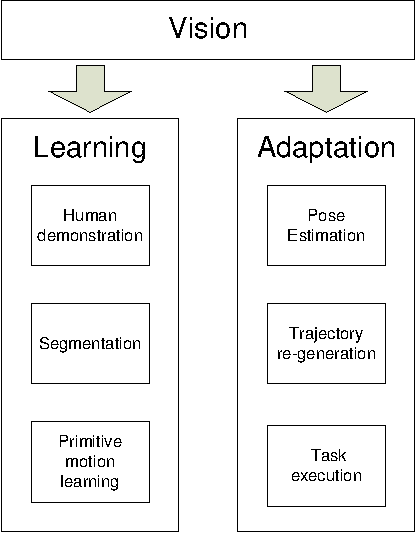
\includegraphics[width=5cm]{./fig/overview.pdf}
\caption{\scriptsize{System overview of bimanual sewing robot}}

\label{fig:overview}
}
\end{figure} 
\section{Experiments}

\subsection{System setup}

\subsection{Human demonstration}

\subsection{Learning}

\subsection{Task execution}

\section{Conclusion} 

In this paper a robotic system for sewing a stent graft is presented. We successfully teach the robot to sew with a curved needle as well as adapt to needle posture changes using a vision guidance system (needle posture re-detection). We analyse the robustness of our method quantitatively by two experiments: fabric piercing and needle regripping, which are the two critical parts for completing one sewing stitch. We show that our system is able to accomplish the sewing task effectively. Our vision system reconstructs the needle shape with sub-millimetres accuracy, and hence is able to guide robustly the robot to sew. The successful rate of our system is over 86$\%$. The failure case is due to the limited workspace caused by the robot joint limit. This problem can be leased by optimizing the task priority in the null space~\cite{yang2015}.

In this study, we use a single robot to manipulate the needle. The successful rate can be improved by using a second robot to cooperate the manipulation. This would make the tasks of both robot easier and also optimize each robot’s joint utilization. Our current system works as an open-loop manner for the needle adaptation part. Tracking the needle in real-time and implementing visual servoing algorithm is desired to increase the sewing accuracy. Further, the sewing presented is conducted in traditional way with needle drivers, in the future, customized sewing device will be designed by us to replace the needle holder to drive the needle performing fine movement. 

The system presented in this paper is a primary and promising study of robot hand sewing. Applications of the presented system and method are not limited only for stent graft sewing; it is also a promising technique for automating robotic suturing.




\bibliographystyle{plain}
\bibliography{ICRA16}


\end{document}
